\begin{figure}[tbp]
\centering
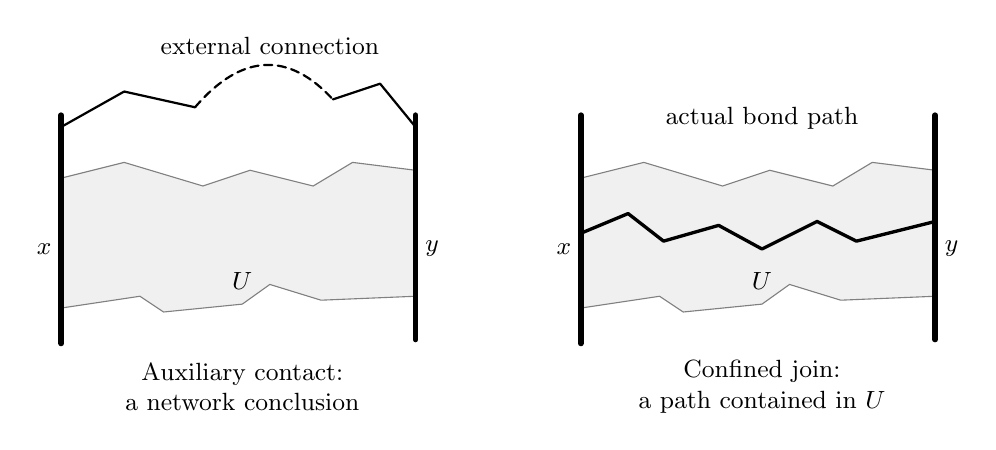
\begin{tikzpicture}[x=1cm,y=1cm,font=\small,line cap=round,line join=round]
  \foreach \shift in {0,6.6} {
    \begin{scope}[xshift=\shift cm]
      \path[fill=gray!12] (0,.75) -- (1,.9) -- (1.3,.7) -- (2.3,.8) -- (2.65,1.05)
        -- (3.3,.85) -- (4.5,.9) -- (4.5,2.5) -- (3.7,2.6) -- (3.2,2.3)
        -- (2.4,2.5) -- (1.8,2.3) -- (.8,2.6) -- (0,2.4) -- cycle;
      \draw[gray] (0,.75) -- (1,.9) -- (1.3,.7) -- (2.3,.8) -- (2.65,1.05)
        -- (3.3,.85) -- (4.5,.9);
      \draw[gray] (0,2.4) -- (.8,2.6) -- (1.8,2.3) -- (2.4,2.5) -- (3.2,2.3)
        -- (3.7,2.6) -- (4.5,2.5);
      \draw[line width=2pt] (0,.3) -- (0,3.2);
      \draw[line width=2pt] (4.5,.35) -- (4.5,3.2);
      \node[left] at (0,1.5) {$x$};
      \node[right] at (4.5,1.5) {$y$};
      \node at (2.3,1.1) {$U$};
    \end{scope}
  }
  \draw[thick] (0,3.05) -- (.8,3.5) -- (1.7,3.3);
  \draw[densely dashed,thick] (1.7,3.3) .. controls (2.3,4) and (2.9,4) .. (3.45,3.4);
  \draw[thick] (3.45,3.4) -- (4.05,3.6) -- (4.5,3.05);
  \node[above] at (2.65,3.85) {external connection};
  \node[align=center] at (2.3,-.25) {Auxiliary contact:\\a network conclusion};
  \draw[line width=1.2pt] (6.6,1.7) -- (7.2,1.95) -- (7.65,1.6) -- (8.35,1.8)
    -- (8.9,1.5) -- (9.6,1.85) -- (10.1,1.6) -- (11.1,1.85);
  \node[above] at (8.9,2.9) {actual bond path};
  \node[align=center] at (8.9,-.25) {Confined join:\\a path contained in $U$};
\end{tikzpicture}
\caption{Network contact and a confined join. The hubs $x,y$ represent
measured blockers or terminal walls, and $U$ is the untouched channel
between them. A network connection may use exterior graph portions
(left). Lemma~\ref{lem:confined-join} produces an actual open path
inside $U$ (right), under its separated-barrier, ordinary-incidence,
and planar-cap hypotheses. In a pure two-end-wire disk, network
connection already has an actual witness; the additional conclusion
here is confinement to the channel.}
\label{fig:actual-network}
\end{figure}
